\batchmode
\makeatletter
\def\input@path{{/Users/vrangbaek/Dropbox/Studieophold/College_of_Europe/Master_Thesis/CoE_thesis_repository//}}
\makeatother
\documentclass{article}\usepackage{graphicx, color}
%% maxwidth is the original width if it is less than linewidth
%% otherwise use linewidth (to make sure the graphics do not exceed the margin)
\makeatletter
\def\maxwidth{ %
  \ifdim\Gin@nat@width>\linewidth
    \linewidth
  \else
    \Gin@nat@width
  \fi
}
\makeatother

\IfFileExists{upquote.sty}{\usepackage{upquote}}{}
\definecolor{fgcolor}{rgb}{0.2, 0.2, 0.2}
\newcommand{\hlnumber}[1]{\textcolor[rgb]{0,0,0}{#1}}%
\newcommand{\hlfunctioncall}[1]{\textcolor[rgb]{0.501960784313725,0,0.329411764705882}{\textbf{#1}}}%
\newcommand{\hlstring}[1]{\textcolor[rgb]{0.6,0.6,1}{#1}}%
\newcommand{\hlkeyword}[1]{\textcolor[rgb]{0,0,0}{\textbf{#1}}}%
\newcommand{\hlargument}[1]{\textcolor[rgb]{0.690196078431373,0.250980392156863,0.0196078431372549}{#1}}%
\newcommand{\hlcomment}[1]{\textcolor[rgb]{0.180392156862745,0.6,0.341176470588235}{#1}}%
\newcommand{\hlroxygencomment}[1]{\textcolor[rgb]{0.43921568627451,0.47843137254902,0.701960784313725}{#1}}%
\newcommand{\hlformalargs}[1]{\textcolor[rgb]{0.690196078431373,0.250980392156863,0.0196078431372549}{#1}}%
\newcommand{\hleqformalargs}[1]{\textcolor[rgb]{0.690196078431373,0.250980392156863,0.0196078431372549}{#1}}%
\newcommand{\hlassignement}[1]{\textcolor[rgb]{0,0,0}{\textbf{#1}}}%
\newcommand{\hlpackage}[1]{\textcolor[rgb]{0.588235294117647,0.709803921568627,0.145098039215686}{#1}}%
\newcommand{\hlslot}[1]{\textit{#1}}%
\newcommand{\hlsymbol}[1]{\textcolor[rgb]{0,0,0}{#1}}%
\newcommand{\hlprompt}[1]{\textcolor[rgb]{0.2,0.2,0.2}{#1}}%

\usepackage{framed}
\makeatletter
\newenvironment{kframe}{%
 \def\at@end@of@kframe{}%
 \ifinner\ifhmode%
  \def\at@end@of@kframe{\end{minipage}}%
  \begin{minipage}{\columnwidth}%
 \fi\fi%
 \def\FrameCommand##1{\hskip\@totalleftmargin \hskip-\fboxsep
 \colorbox{shadecolor}{##1}\hskip-\fboxsep
     % There is no \\@totalrightmargin, so:
     \hskip-\linewidth \hskip-\@totalleftmargin \hskip\columnwidth}%
 \MakeFramed {\advance\hsize-\width
   \@totalleftmargin\z@ \linewidth\hsize
   \@setminipage}}%
 {\par\unskip\endMakeFramed%
 \at@end@of@kframe}
\makeatother

\definecolor{shadecolor}{rgb}{.97, .97, .97}
\definecolor{messagecolor}{rgb}{0, 0, 0}
\definecolor{warningcolor}{rgb}{1, 0, 1}
\definecolor{errorcolor}{rgb}{1, 0, 0}
\newenvironment{knitrout}{}{} % an empty environment to be redefined in TeX

\usepackage{alltt}
\usepackage[T1]{fontenc}
\usepackage[latin9]{inputenc}
\usepackage[a4paper]{geometry}
\geometry{verbose,tmargin=2.5cm,bmargin=2.5cm,lmargin=3cm,rmargin=2.5cm}
\setcounter{secnumdepth}{2}
\setcounter{tocdepth}{2}
\usepackage{varioref}
\usepackage{amstext}
\usepackage{setspace}
\usepackage[authoryear]{natbib}
\onehalfspacing
\usepackage[unicode=true]
 {hyperref}

\makeatletter
\@ifundefined{date}{}{\date{}}
%%%%%%%%%%%%%%%%%%%%%%%%%%%%%% User specified LaTeX commands.
%\SweaveOpts{results='asis', echo=FALSE} % Controls global Sweave/knitr options
%\usepackage{knitr}
\usepackage{rotating}
\usepackage{longtable}

\makeatother

\begin{document}

\title{Master Thesis}


\author{A.V. RIIS}


\date{2013}

\maketitle
\newpage{}


\section*{Statutory Declaration}

I hereby declare that the thesis has been written by myself without
any external unauthorised help, that it has been neither presented
to any institution for evaluation nor previously published in its
entirety or in parts. Any parts, words or ideas, of the thesis, however
limited, and including tables, graphs, maps etc., which are quoted
from or based on other sources have been acknowledged as such without
exception.

\newpage{}
\begin{abstract}
Abstract
\end{abstract}
\newpage{}


\section*{Keywords}
\begin{itemize}
\item economic growth
\item institional measures
\item political constraints
\end{itemize}
\pagebreak{}

\tableofcontents{}







\pagebreak{}


\section{Introduction}

This project will look further into the institutional determinants
of economic progress. The main econometric models attempt to replicate
the findings of Henisz (2000). This project will use the standard
linear pooled model, GLS and GMM to attempt to determine how institutions
and political constraints influence economic growth of countries by
using a variety of institutional measures.
\begin{quote}
\textquotedblleft{}(...) many politicians are being shockingly irresponsible.
In different ways, politicians\textquoteright{} actions (or inaction)
are the biggest short-term danger facing the American, European and
Chinese economies. Judging by politicians\textquoteright{} current
behaviour, the world economy could slow a lot further. It could even
tip into recession in 2013.\textquotedblright{}%
\footnote{\textquoteleft{}The World Economy: Investors, Beware\textquoteright{},
The Economist, 6 October 2012, \href{http://www.economist.com/node/21564232}{http://www.economist.com/node/21564232}. %
}
\end{quote}

\section{Hypothesis, Research Question and Scope of Paper}

The underlying assumption of this paper is that the political organization
of a given country has a significant influence on the degree to which
this country experiences economic growth and development. Moreover,
it is hypothesised that certain political constraints can be identified
in order to pinpoint how, if at all, political organization in this
sense is related to economic growth.


\section{Literature Review}

Determining which way the causality runs when looking at the influence
of institutions on economic growth is a contentious topic. The question
is whether democratic institutions cause economic growth, i.e. that
countries with a higher degree of democracy are more prone to economic
progress compared to countries with more autocratic characteristics,
or whether countries that are more economically developed are more
likely to foster democratic institutions. A simple, but compelling
test can be undertaken by looking at the Korean Peninsula. Looking
at the divergent paths of North and South Korea there is evidence
that democratic institutions cause economic growth and not vice versa.
Economic progress of South Korea result of institutional path choosen
after the end of the war in 1953 \citep[p. 272]{glaeser2004doinstitutions}.

Another topic that is important to tackle in understanding the institutional
influence on economic growth is how institutions are measured. Glaeser
et al. (2004) looks at three measures of institutions, namely risk
of appropriation, quality of government and constraints on the executive.

However, even before one decides on how to measures institutions,
they must defined. A concise and precise notion of instutions is that
they are in essence constraints (North 1981, quoted in Glaeser et
al. 2004) and that they are permanent or stable (Glaeser et al. 2004,
quoted in Voigt, 2013, p. 3). The frequently used measures such as
those from the International Country Risk Guide, the Governance Indicators
from the World Bank \citep{kaufmann2010theworldwide} and the Polity
IV measures. Glaeser et al. argues that these do neither measure the
stability of institutions nor their constraints, but only policy outcomes
\citet[p. 4]{voigt2013hownot}.

Another terminological distinction is between economic and political
institutions. Voigt (2013, p. 7) proposes to see economic institutions
as enabling and political institutions as constraining. Institutions
can also be formal or informal, public or private, \emph{de jure }or
\emph{de facto}, internal or external\emph{ }(Voigt, 2013, pp. 6-8).
Institutions also increase the level of predictability in a given
society given incentives to make long-term investments.

Human capital and constraints on the executive are both associated
with economic growth, but Glaeser et al. argues that human capital
is a stronger predictor. The two might however be related as higher
levels of education in a given society could result in electoral demands
that the executive be further constrained... 

\citet{voigt2013hownot} looks at how institutions should not be measured
and presents a number of proposals on how to measure institutions.
Voigt raises four points concerning the measurement of institutions
of which two are worth mentioning:
\begin{enumerate}
\item the traditional aggregate measures such as \textquoteleft{}the rule
of law\textquoteright{} are too vague to contain meaningful information,
so measures of institutions should refer to specific institutions;
and
\item although many established measures of institutions are subjective
such as the World Bank indicators and the Quality of Government indicators,
the objective measures are generally preferable.
\end{enumerate}
Moreover, to summarise the current consensus on the topic, the paper
proposes that ``institutions matter crucially for economic development''
\citeyearpar[p. 1]{voigt2013hownot}.

One of the conclusions of Glaeser et al. (2004) is that some of the
work purporting to measure the influence of institutions on economic
growth has not measured institutions, but rather policies \citep[p. 2]{voigt2013hownot}.

Another controversy in the literature concerns whether democratic
institutions serve as mechanims for ensuring property rights, thus
encouraging investment and economic growth, or whether increased levels
of human capital lead to democratic institutions. In essence, the
question is whether democratic institutions are the cause or consequence
of economic growth. This is at least how the controversy is presented
in Voigt (2013). On closer inspection the argument seems to lend itself
to another interpretation, namely that the views are in fact not conflicting,
but complementary: it might both be true that human capital lead to
democratic institutions and that democratic institutions lead to economic
growth. The relevant question is rather whether democratic institutions
lead to higher levels of human capital or vice versa.

Human capital and democratic institutions understood as constraints
on the executive are both associated with economic growth, but Glaeser
et al. (2004) argues that human capital is a stronger predictor, although
they do not discredit the other camp that purports that democratic
institutions are the main predictor \citep[p. 3]{voigt2013hownot}.
Glaeser et al. (2004) challenges the use of instrumental variables
used in the works by Acemoglu among others to predict economic development
of settler colonies in the US. They argue that human capital is a
more reliable predictor of economic growth than institutions per se.
The settlers brought themselves rather than their institutions.

``Many creators of indicators seem to assume simple linear relationships
between an institution and some outcome'' \citep[p. 10]{voigt2013hownot}.

More than one institution is likely to affect observed outcome, so
excluding any one aspect would result in omitted variable bias \citep[p. 11]{voigt2013hownot}.

In situations where there are repeat interactions, internal institution
trump state-run ones. Confidence (\emph{tillid}) argument...

Political constraints might also have other effects than contributing
to economic progress and development. \citet{fatas2003thecase} explores
the effects of discretionary fiscal policy on output volatility and
economic growth and concludes, inter alia, that \textquotedblleft{}prudent
use of fiscal policy is explained to a large extent by the presence
of political constraints and other political and institutional variables.
 If discretionary fiscal policy has an effect on economic growth,
but fiscal policy is in turn influenced by the level of political
constraints, then we have to be careful to bear in mind that there
is an intermediating factor in the relationship between political
constraints and economic growth.

Economic progress is most probably determined by a confluence of factors,
but this project aims at looking at institutional variables such as
the degree of political constraints and some of measures of institutional
quality.

This paper will use the dataset constructed by W.J. Henisz and is
called POLCONIII and POLCONV. This dataset is time series data with
measures of political constraints from all countries in the world.
This data will then be used as the independent variable, while different
economic variables such as growth, unemployment, government debt etc.
will be used as the dependent variable. Control variables will include
measures of social capital as by \citet{barro1996democracy}.

The political constraints variable is defined as the number of independent
veto points over policy outcomes and the distribution of preferences
of the actors that inhabit these veto points. The variable is calculated
as one minus the expected range of policies for which a change in
the status quo can be agreed upon by veto power. An unchecked executive
can always obtain policy $X_{E}$ and is thus guaranteed their maximum
utility of 0. Political constraints are thus measures as (1 \textendash{}
political discretion) = 0 in the extreme case of full discretion (=1). 

Initially, we attempt a standard linear model pooling all the data
across countries and years, which can be written as 
\[
y_{it}=\alpha+\beta^{T}x_{it}+u_{it},
\]


where $i=1,...,n$ is the country index, $t=1,...T$ is the time index
and $u_{it}$ a random disturbance term with mean 0 \citep[p. 2]{croissant2008paneldata}.


\section{Data}

The panel data set used is an unbalanced panel and made up from a
number of sources, which are explained below.


\subsection{Variables}

The variables used are primarily taken from Table 3 in Henisz (2000)
and include:
\begin{itemize}
\item Real Per Capita GDP Growth 
\item Male Secondary Education (years) 
\item Female Secondary Education (years) 
\item Log(Life Expectancy) 
\item Log(Fertility Rate) 
\item Government Consumption (\% GDP) 
\item Log(Black Market Exchange Rate Premium)
\item Change in the Terms of Trade
\item Total Investment (\% GDP) 
\item Log(Law \& Order Index)
\item Democracy Index 
\item Political Constraint Index (POLCON) 
\item Political Constraint Index (POLCONJ)
\end{itemize}
In the subsections below, I will outline how and where the data is
found, possibly transformed and what the existing literature has to
say on the topic. Table \ref{tabsmall} on page \pageref{tabsmall}
gives some summary statistics of all the variables included, so if
there is no table included in the subsections below, this table can
be consulted for more information on the variable.


\subsubsection{Measures on political constraints\label{sub:Measures-of-POLCON}}




The political constraints variable is defined as the number of independent
veto points over policy outcomes and the distribution of preferences
of the actors that inhabit these veto points. The variable is calculated
as one minus the expected range of policies for which a change in
the status quo can be agreed upon by veto power. An unchecked executive
can always obtain policy XE and is thus guaranteed their maximum utility
of 0. Political constraints are thus measures as (1 \textendash{}
political discretion) = 0 in the extreme case of full discretion (=1)
\citep{henisz2000theinstitutional}. We expect that there is a positive
relationship between the degree of political constraints and economic
growth. This is supported by the results of Henisz (2000).

Table \ref{POLCON_tab} on page \pageref{POLCON_tab} shows the some
summary statistics of the different variations of this variable. The
earliest observation is from 1800, while the
newest is from 2007. POLCONIII is available for
226 countries. The difference between POLCONIII and POLCONV is that
the latter includes two additional veto points (the judiciary and
the subfederal entities). POLCONV is available for 200 countries.

% latex table generated in R 2.15.2 by xtable 1.7-1 package
% Sat Mar 30 14:10:41 2013
\begin{table}[ht]
\centering
\begin{tabular}{rrrrrrr}
  \hline
 & n & mean & median & min & max & stdev \\ 
  \hline
POLCONIII & 14923.00 & 0.16 & 0.00 & 0.00 & 0.73 & 0.21 \\ 
  POLCONV & 7179.00 & 0.30 & 0.12 & 0.00 & 0.90 & 0.33 \\ 
  POLCONVJ & 5151.00 & 0.12 & 0.00 & 0.00 & 0.86 & 0.22 \\ 
   \hline
\end{tabular}
\caption{Descriptive statistics of the variables on political constraints (Henisz 2000)} 
\label{POLCON_tab}
\end{table}



The POLCON measures are strongly correlated with the ICRG risk indices
\citep[p. 10]{henisz2000theinstitutional}.
\begin{quotation}
``POLCON and POLCONJ differ in that the latter uses actual data on
the appointment history of High Court justices to compute the alignment
and fractionalization of the High Court.''\citep[p. 10]{henisz2000theinstitutional}
\end{quotation}
As Henisz (2000) notes himself is the assumptions underlysing this
measure quite strong and unrealistic, but they should however be regarded
as a rough proxy of political constraints.


\subsubsection{Measures of real GDP per capita\label{sub:Measures-of-gdp}}

Henisz (2000) uses some the same data as \citet{barro1996democracy},
who has used GDP figures from the Summers-Heston data set, or Penn
World Table (PWT) \citep{heston2012pennworld}. Barro (1996) uses
GDP figures from version 5.5 of the Penn World Table, while I will
be using the newest version 7.1. To avoid confusion it should be noted
that in these data sets ``real'' means ``PPP converted'' instead
of ``in constant price''. The variable used is \emph{rgdpl} and
the code book describes it as PPP Converted GDP Per Capita (Laspeyres),
derived from growth rates of c, g, i, at 2005 constant prices. The
growth rate is then calculated using the formula 
\[
\hat{w}_{t}=\frac{x_{t}-x_{t-1}}{x_{t-1}},
\]
 where $\hat{w}_{t}$ is real GDP growth rate for year $t$ and $x_{t}$
are GDP levels at year $t$ \citep{universityofzurich2010logarithms}.

The validity of the Penn World Table is discussed in \citet{johnson2009isnewer2}
who demonstrate that the measures of GDP growth for the same country
at the same point in time changes across successive versions of the
data set. They propose that more ``robust results by using national
accounts data, even though they are not PPP-adjusted.'' For practical
reasons this is not possible in this project, so I will still be using
the PWT data.

Another measures of GDP growth is found in the Global Development
Network Growth Database \citep{easterly2001globaldevelopment}. For
practical reasons, this measure is used instead.

As \citet[p. 4]{barro1996democracy} writes the neoclassical model
of economic growth predicts that GDP growth is negatively correlated
with the initial level of GDP. 
\begin{quote}
``Empirically, the initial level of per capita GDP enters into the
growth equation in the form $\text{log}(y_{t-1})$ so that the coefficient
on this variable represents the rate of convergence, that is, the
responsiveness of the growth rate, $Dy_{t}$, to a proportional change
in $y_{t-1}$.''\citep[p. 237]{barro2003determinants}
\end{quote}
The convergence effect is ``conditional on the starting amount of
human capital in the forms of educational attainment and life expectancy
and on a set of explanatory variables that capture policies and national
characteristics'' \citep[p. 273]{barro2003determinants}.

\begin{knitrout}
\definecolor{shadecolor}{rgb}{0.969, 0.969, 0.969}\color{fgcolor}\begin{kframe}


{\ttfamily\noindent\color{warningcolor}{\#\# Warning: NaNs produced}}\end{kframe}
\end{knitrout}



\subsubsection{Measures of educational attainment}

Data on educational attainment is from the Barro-Lee Educational Attainment
Dataset \citep{barro2010anew}. Henisz \citeyearpar{henisz2000theinstitutional}
mentions that he has his educational attainment data from \citet{barro1994sources},
who only uses information on schooling of the adult population aged
25 and above, but acknowledges in a footnote that this is unfortunate
as ``much of the labor force in developing countries consists of
younger persons.`` However, the newer data sets include information
on schooling of the population aged 15 and above. The data set only
has data from every fifth year.





\subsubsection{Measures on life expectancy}

As mentioned in \citet[p. 11]{barro1994sources} the data on life
expectancy is from the UN. The data in this report, however, is taken
from the World Bank indicator SP.DYN.LE00.IN with the name ``Life
expectancy at birth, total (years)''.%
\footnote{From the source notes: Life expectancy at birth indicates the number
of years a newborn infant would live if prevailing patterns of mortality
at the time of its birth were to stay the same throughout its life.
Derived from male and female life expectancy at birth from sources
such as: (1) United Nations Population Division. World Population
Prospects, (2) United Nations Statistical Division. Population and
Vital Statistics Reprot (various years), (3) Census reports and other
statistical publications from national statistical offices, (4) Eurostat:
Demographic Statistics, (5) Secretariat of the Pacific Community:
Statistics and Demography Programme, and (6) U.S. Census Bureau: International
Database.%
}





\subsubsection{Measures on fertility rates}

The indicator is taken from the World Bank (indicator SP.DYN.TFRT.IN)
and is described as: Fertility rate, total (births per woman).%
\footnote{\href{http://data.worldbank.org/indicator/SP.DYN.TFRT.IN}{http://data.worldbank.org/indicator/SP.DYN.TFRT.IN}%
} Moreover, the ``total fertility rate represents the number of children
that would be born to a woman if she were to live to the end of her
childbearing years and bear children in accordance with current age-specific
fertility rates.''





\subsubsection{Government Consumption (\% GDP)}

This measures is also taken from the Penn World Table. The variable
is called \emph{kg} and is described as Government Consumption Share
of PPP Converted GDP Per Capita at 2005 constant prices (\%). The
basic descriptive statistics are reported in table \ref{kg_tab}.

The influence of government expenditure on economic growth is a contentious
topic. \citet{barro1991government}, the seminal article on the topic,
found a negative relationship between government consumption and economic
growth, which the results in this project also find (see table \ref{tab:fe3}
on page \pageref{tab:fe3}).

% latex table generated in R 2.15.2 by xtable 1.7-1 package
% Sat Mar 30 14:10:44 2013
\begin{table}[ht]
\centering
\begin{tabular}{rrrrrrr}
  \hline
 & n & mean & median & min & max & stdev \\ 
  \hline
kg & 8940.00 & 11.86 & 8.89 & 0.31 & 67.19 & 8.97 \\ 
   \hline
\end{tabular}
\caption{Descriptive statistics of Government Consumption} 
\label{kg_tab}
\end{table}




\subsubsection{Black Market Exchange Rate Premium}

These measures come originally from \citet{wood1991globaltrends},
but has been found using \citet{easterly2001globaldevelopment}.%
\footnote{From the source notes of the Easterly (2001): Levine and Renelt; World's
Currency Yearbook (for 1985, 1990-93); Adrian Wood, Global trends
in real exchange rates: 1960-84, WB Discussion paper no. 35. 1988
(filling in missing observations); Global Development Finance \& World
Development Indicators (for 1996-1997, calculated as (parallel Xrate/official
Xrate-1){*}100); values for industrial countries are added as 0).%
} Two values have been changed from the originally downloaded data
set, namely the observations for Myanmar and Iraq in 1999 because
it said ``Err:520''. The data set has been downloaded as and xls
file and then converted to a csv file before imported into the statistics
programme. 

The variable has been log-transformed. As we can see in figure \ref{fig:bmp_tab}
on page \pageref{fig:bmp_tab}, the variable appears normally distributed
after the log-transformation. In table \ref{bmp_tab} on page \pageref{bmp_tab},
we see the summary statistics of the variable before and after the
log-transformation.

\citet{barnett1999inflation} writes that ``the black market premium
is intended to serve as a measure of market distortions more broadly
defined, and there appears to be a small but significant negative
relationship between economic growth and the black market premium.''
\citet[p. 13]{barro1994sources} writes:
\begin{quote}
``We view the black-market premium on foreign exchange as a proxy
for market distortions, whether due to exogenous government policies
or to reactions to external shocks, such as changes in the terms of
trade. (The black-market premium is also a desirable variable because
it is objectively measurable and widely available.) Thus, we anticipate
that a higher black-market premium, like other governmental distortions,
lowers the steady-state level of output per effective worker and therefore
reduces the growth rate for given values of the state variables.''
\end{quote}
\citet{emran2004isblack} has however cast some doubt on the validity
of this indicator of the equilibrium exchange rate by using data from
South East Asia to reject the null hypothesis that there is a relationship.

\begin{knitrout}
\definecolor{shadecolor}{rgb}{0.969, 0.969, 0.969}\color{fgcolor}\begin{kframe}


{\ttfamily\noindent\color{warningcolor}{\#\# Warning: NaNs produced}}\end{kframe}
\end{knitrout}

% latex table generated in R 2.15.2 by xtable 1.7-1 package
% Sat Mar 30 14:10:44 2013
\begin{table}[ht]
\centering
\begin{tabular}{rrrrrrr}
  \hline
 & n & mean & median & min & max & stdev \\ 
  \hline
bmp & 4462.00 & 299.86 & 4.84 & -89.16 & 413361.08 & 8918.95 \\ 
  lbmp & 4196.00 & -Inf & 1.80 & -Inf & 12.93 &  \\ 
   \hline
\end{tabular}
\caption{Descriptive statistics of the variables on black market premium} 
\label{bmp_tab}
\end{table}
\begin{figure}[]


{\centering 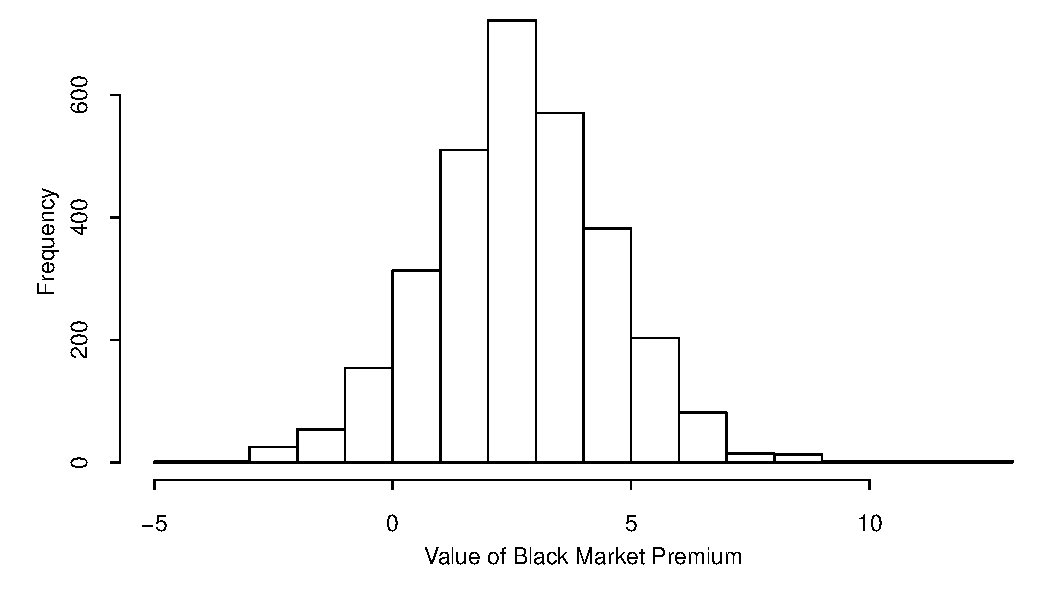
\includegraphics[width=.9\linewidth]{figure/bmp_tab} 

}

\caption[Histogram of log(Black Market Premium)]{Histogram of log(Black Market Premium)\label{fig:bmp_tab}}
\end{figure}





\subsubsection{Change in the Terms of Trade}

This measure is also taken from \citet{easterly2001globaldevelopment}.\citet[p. 531]{barro2004economic}
have found a positive and significant relationship between between
terms of trade measures and economic growth, while \citet[p. 24]{barro1994sources}
finds a positive, but insignificant relationship. The variable is
named \emph{ToT}.





\subsubsection{Total Investment (\% GDP)}

This measures is also taken from the Penn World Table. The variable
is called \emph{ki} and is described as Investment Share of PPP Converted
GDP Per Capita at 2005 constant prices (\%).


\subsubsection{Law \& Order Index}

The Law \& Order Index is provided by POLCON data set. Another measure
from the ICRG has also been included, namely the mean value of the
ICRG variables \textquotedblleft{}Corruption\textquotedblright{},
\textquotedblleft{}Law and Order\textquotedblright{} and \textquotedblleft{}Bureaucracy
Quality\textquotedblright{}, scaled 0-1 from the Quality of Government
Dataset \citep{teorell2011thequality}.







\subsubsection{Democracy Index}

This variable \emph{democ }is from Polity data set \citep{marshall2011polityiv}.
The values -66, -77 and -88 are removed from the dataset.








\subsection{Data Description}

The entire set of variables can be seen in table \ref{tabsmall} (see
p. \pageref{tabsmall}). Here the mean, median, minimum, maximum and
standard deviation values are reported.

\begin{singlespace}
\begin{flushleft}


\par\end{flushleft}
\end{singlespace}

% latex table generated in R 2.15.2 by xtable 1.7-1 package
% Sat Mar 30 14:10:46 2013
\begin{sidewaystable}[ht]
\centering
\begin{tabular}{rrrrrrr}
  \hline
 & n & mean & median & min & max & stdev \\ 
  \hline
POLCONIII & 2297.00 & 0.21 & 0.10 & 0.00 & 0.71 & 0.23 \\ 
  POLCONV & 2270.00 & 0.30 & 0.14 & 0.00 & 0.89 & 0.34 \\ 
  POLCONVJ & 1821.00 & 0.16 & 0.00 & 0.00 & 0.86 & 0.25 \\ 
  Law...Order..from.ICRG. & 864.00 & 3.62 & 4.00 & 1.00 & 6.00 & 1.57 \\ 
  llaw.order & 864.00 & 1.17 & 1.39 & 0.00 & 1.79 & 0.53 \\ 
  rgdpl & 2147.00 & 7346.44 & 4102.69 & 240.57 & 60412.86 & 8277.19 \\ 
  kg & 2147.00 & 11.01 & 8.52 & 2.26 & 49.37 & 7.64 \\ 
  ki & 2147.00 & 22.96 & 21.24 & 0.73 & 80.39 & 10.74 \\ 
  inigdp & 2311.00 & 4328.19 & 2622.31 & 218.89 & 44566.52 & 5847.67 \\ 
  gdp.growth & 1962.00 & 1.55 & 2.02 & -52.07 & 110.84 & 6.54 \\ 
  lgdp.growth & 1376.00 & 1.05 & 1.22 & -4.03 & 4.71 & 1.01 \\ 
  yr.sch.secF & 377.00 & 1.40 & 1.10 & 0.01 & 5.36 & 1.19 \\ 
  yr.sch.secM & 377.00 & 1.72 & 1.49 & 0.04 & 5.39 & 1.16 \\ 
  lexpec & 2310.00 & 61.75 & 64.43 & 26.82 & 80.57 & 11.24 \\ 
  llexpec & 2310.00 & 4.10 & 4.17 & 3.29 & 4.39 & 0.20 \\ 
  fert & 2313.00 & 4.51 & 4.51 & 1.17 & 8.29 & 2.02 \\ 
  lfert & 2313.00 & 1.38 & 1.51 & 0.16 & 2.12 & 0.52 \\ 
  bmp & 1784.00 & 673.22 & 6.00 & -57.36 & 413361.08 & 14093.00 \\ 
  lbmp & 1703.00 & -Inf & 1.99 & -Inf & 12.93 &  \\ 
  ToT & 1597.00 & 111.89 & 102.19 & 43.52 & 309.49 & 32.09 \\ 
  icrgQoG & 842.00 & 0.56 & 0.55 & 0.11 & 1.00 & 0.22 \\ 
  l.icrgQoG & 842.00 & -0.67 & -0.59 & -2.20 & 0.00 & 0.47 \\ 
  democ & 2313.00 & 3.99 & 2.00 & 0.00 & 10.00 & 4.27 \\ 
   \hline
\end{tabular}
\caption{Descriptive statistics of the variables used} 
\label{tabsmall}
\end{sidewaystable}




\section{Statistical Model}

The first type of estimation that will be used is fixed effects estimation,
where the unobserved effects are removed by averaging the model over
time and thus transformed into time-demeaned data \citep[pp. 481-2]{wooldridge2009introductory}. 

With fixed effects we allow the intercept to vary with group, or time,
or both, while the other parameters are generally still assumed to
be homogeneous \citep[p. 42]{croissant2008paneldata}.


\section{Estimation and Misspecification Testing}


\subsection{Estimation Results}

In table \ref{tab:fe3} on page \pageref{tab:fe3}, we see the results
of fixed effects estimation with individual effects. Here we estimate
the relationship between the measure of political constraints POLCONV
allowing for individual-specific, time-invariant effects. Models (2)
through (6) use individual-specific, time-invariant effects to estimate
the different measures of political constraints and institutions.
As we can see the only other significant indicator is the democracy
indicator from the PolityIV data set. The law \& order measure and
the risk measure from ICRG are only available for few countries, so
the number of observations drops significantly. Most of the coefficients
correspond to the findings of Henisz (2000).

In table \ref{tab:fe4} on page \pageref{tab:fe4}, we allow for both
individual and time effects. Going from one to other does not change
the sign of any of the variables, but some of the significance levels
change, e.g. terms of trade becomes significant. Finally, we produce
the results using only time effects in table \ref{tab:fe5} on page
\pageref{tab:fe5} and pooled regression results in table \ref{tab:fe6}
on page \pageref{tab:fe6}.



\def\sym#1{\ifmmode^{#1}\else\(^{#1}\)\fi}
\begin{sidewaystable}[p]
\centering
\small
\begin{tabular}{l*{6}{c}}
\hline\hline
	 &\multicolumn{1}{c}{( 1 )}  	 &\multicolumn{1}{c}{( 2 )}  	 &\multicolumn{1}{c}{( 3 )}  	 &\multicolumn{1}{c}{( 4 )}  	 &\multicolumn{1}{c}{( 5 )}  	 &\multicolumn{1}{c}{( 6 )}  \\  &\multicolumn{1}{c}{lgdp.growth} &\multicolumn{1}{c}{lgdp.growth} &\multicolumn{1}{c}{lgdp.growth} &\multicolumn{1}{c}{lgdp.growth} &\multicolumn{1}{c}{lgdp.growth} &\multicolumn{1}{c}{lgdp.growth} \\
\hline
yr.sch.secF 		&-1.411 		&-1.62 		&-1.847\sym{*} 		&-1.314 		&-2.528 		&-5.843 \\
  		&(0.97) 		&(0.991) 		&(1.077) 		&(0.99) 		&(8.717) 		&(8.365) \\
yr.sch.secM 		&2.068\sym{**} 		&2.143\sym{**} 		&2.424\sym{***} 		&1.935\sym{**} 		&2.18 		&4.481 \\
  		&(0.843) 		&(0.869) 		&(0.894) 		&(0.861) 		&(10.285) 		&(9.943) \\
lbmp 		&0.047 		&0.03 		&0.008 		&0.026 		&-0.344 		&-0.455 \\
  		&(0.077) 		&(0.079) 		&(0.08) 		&(0.075) 		&(0.205) 		&(0.262) \\
lfert 		&-0.124 		&-0.287 		&-0.554 		&-0.38 		&-0.842 		&-4.821 \\
  		&(1.188) 		&(1.21) 		&(1.239) 		&(1.152) 		&(9.192) 		&(10.288) \\
kg 		&-0.016 		&-0.017 		&-0.013 		&-0.017 		&0.128 		&-0.104 \\
  		&(0.054) 		&(0.055) 		&(0.056) 		&(0.054) 		&(0.574) 		&(0.618) \\
ki 		&0.009 		&0.009 		&0.011 		&0.004 		&0.159 		&0.183 \\
  		&(0.021) 		&(0.022) 		&(0.023) 		&(0.022) 		&(0.101) 		&(0.125) \\
llexpec 		&-6.382\sym{*} 		&-6.54\sym{*} 		&-7.874\sym{**} 		&-6.941\sym{**} 		&-13.822 		&-20.849 \\
  		&(3.263) 		&(3.358) 		&(3.417) 		&(3.237) 		&(19.534) 		&(22.165) \\
ToT 		&-0.003 		&-0.004 		&-0.004 		&-0.002 		&-0.006 		&-0.007 \\
  		&(0.005) 		&(0.005) 		&(0.005) 		&(0.005) 		&(0.023) 		&(0.022) \\
POLCONV 		&-1.092\sym{*} 		& 		& 		& 		& 		& \\
  		&(0.564) 		& 		& 		& 		& 		& \\
POLCONIII 		& 		&-0.857 		& 		& 		& 		& \\
  		& 		&(0.898) 		& 		& 		& 		& \\
POLCONVJ 		& 		& 		&0.03 		& 		& 		& \\
  		& 		& 		&(1.026) 		& 		& 		& \\
democ 		& 		& 		& 		&-0.084\sym{*} 		& 		& \\
  		& 		& 		& 		&(0.045) 		& 		& \\
llaw.order 		& 		& 		& 		& 		&-1.228 		& \\
  		& 		& 		& 		& 		&(1.321) 		& \\
l.icrgQoG 		& 		& 		& 		& 		& 		&-1.974 \\
  		& 		& 		& 		& 		& 		&(2.019) \\
\hline
$R^2$ 		&0.182 		&0.149 		&0.15 		&0.179 		&0.843 		&0.893 \\
$adj.R^2$ 		&0.113 		&0.092 		&0.093 		&0.112 		&0.067 		&0.05 \\
$N$ 		&\multicolumn{1}{c}{110} 		&\multicolumn{1}{c}{110} 		&\multicolumn{1}{c}{104} 		&\multicolumn{1}{c}{111} 		&\multicolumn{1}{c}{38} 		&\multicolumn{1}{c}{36} \\
\hline\hline
\multicolumn{7}{l}{\footnotesize Standard errors in parentheses}\\
\multicolumn{7}{l}{\footnotesize $^{*}$ (p $\le$ 0.1), $^{**}$ (p $\le$ 0.05), $^{***}$ (p $\le$ 0.01)}\\
\end{tabular}
\caption{Estimation results from fixed effects estimation (individual effects)}
\label{tab:fe3}
\end{sidewaystable}
\def\sym#1{\ifmmode^{#1}\else\(^{#1}\)\fi}
\begin{sidewaystable}[p]
\centering
\small
\begin{tabular}{l*{6}{c}}
\hline\hline
	 &\multicolumn{1}{c}{( 1 )}  	 &\multicolumn{1}{c}{( 2 )}  	 &\multicolumn{1}{c}{( 3 )}  	 &\multicolumn{1}{c}{( 4 )}  	 &\multicolumn{1}{c}{( 5 )}  	 &\multicolumn{1}{c}{( 6 )}  \\  &\multicolumn{1}{c}{lgdp.growth} &\multicolumn{1}{c}{lgdp.growth} &\multicolumn{1}{c}{lgdp.growth} &\multicolumn{1}{c}{lgdp.growth} &\multicolumn{1}{c}{lgdp.growth} &\multicolumn{1}{c}{lgdp.growth} \\
\hline
yr.sch.secF 		&-0.901 		&-0.985 		&-1.19 		&-0.834 		&-1.491 		&-2.668 \\
  		&(0.985) 		&(0.999) 		&(1.09) 		&(1.004) 		&(5.305) 		&(7.517) \\
yr.sch.secM 		&2.778\sym{***} 		&2.937\sym{***} 		&3.144\sym{***} 		&2.756\sym{***} 		&7.106 		&9.473 \\
  		&(0.89) 		&(0.905) 		&(0.928) 		&(0.913) 		&(6.548) 		&(9.269) \\
lbmp 		&0.033 		&0.015 		&0.01 		&0.016 		&-0.158 		&-0.106 \\
  		&(0.081) 		&(0.081) 		&(0.082) 		&(0.078) 		&(0.145) 		&(0.345) \\
lfert 		&-0.899 		&-1.159 		&-1.409 		&-1.104 		&2.35 		&3.563 \\
  		&(1.246) 		&(1.242) 		&(1.309) 		&(1.213) 		&(5.723) 		&(10.808) \\
kg 		&0.06 		&0.067 		&0.068 		&0.062 		&0.837 		&0.961 \\
  		&(0.061) 		&(0.061) 		&(0.063) 		&(0.061) 		&(0.451) 		&(0.96) \\
ki 		&0.016 		&0.018 		&0.018 		&0.013 		&0.225\sym{*} 		&0.214 \\
  		&(0.023) 		&(0.023) 		&(0.024) 		&(0.023) 		&(0.067) 		&(0.109) \\
llexpec 		&-3.586 		&-3.602 		&-4.125 		&-3.435 		&3.397 		&1.594 \\
  		&(3.838) 		&(3.887) 		&(4.083) 		&(3.794) 		&(13.735) 		&(25.36) \\
ToT 		&-0.009\sym{*} 		&-0.01\sym{*} 		&-0.01\sym{*} 		&-0.008 		&-0.027 		&-0.032 \\
  		&(0.005) 		&(0.005) 		&(0.005) 		&(0.005) 		&(0.016) 		&(0.026) \\
POLCONV 		&-0.716 		& 		& 		& 		& 		& \\
  		&(0.606) 		& 		& 		& 		& 		& \\
POLCONIII 		& 		&-0.347 		& 		& 		& 		& \\
  		& 		&(0.912) 		& 		& 		& 		& \\
POLCONVJ 		& 		& 		&0.321 		& 		& 		& \\
  		& 		& 		&(1.076) 		& 		& 		& \\
democ 		& 		& 		& 		&-0.05 		& 		& \\
  		& 		& 		& 		&(0.047) 		& 		& \\
llaw.order 		& 		& 		& 		& 		&-0.167 		& \\
  		& 		& 		& 		& 		&(0.909) 		& \\
l.icrgQoG 		& 		& 		& 		& 		& 		&0.334 \\
  		& 		& 		& 		& 		& 		&(2.447) \\
\hline
$R^2$ 		&0.236 		&0.221 		&0.224 		&0.233 		&0.957 		&0.954 \\
$adj.R^2$ 		&0.135 		&0.127 		&0.127 		&0.135 		&0.05 		&0.027 \\
$N$ 		&\multicolumn{1}{c}{110} 		&\multicolumn{1}{c}{110} 		&\multicolumn{1}{c}{104} 		&\multicolumn{1}{c}{111} 		&\multicolumn{1}{c}{38} 		&\multicolumn{1}{c}{36} \\
\hline\hline
\multicolumn{7}{l}{\footnotesize Standard errors in parentheses}\\
\multicolumn{7}{l}{\footnotesize $^{*}$ (p $\le$ 0.1), $^{**}$ (p $\le$ 0.05), $^{***}$ (p $\le$ 0.01)}\\
\end{tabular}
\caption{Estimation results from fixed effects estimation (individual and time effects)}
\label{tab:fe4}
\end{sidewaystable}
\def\sym#1{\ifmmode^{#1}\else\(^{#1}\)\fi}
\begin{sidewaystable}[p]
\centering
\small
\begin{tabular}{l*{6}{c}}
\hline\hline
	 &\multicolumn{1}{c}{( 1 )}  	 &\multicolumn{1}{c}{( 2 )}  	 &\multicolumn{1}{c}{( 3 )}  	 &\multicolumn{1}{c}{( 4 )}  	 &\multicolumn{1}{c}{( 5 )}  	 &\multicolumn{1}{c}{( 6 )}  \\  &\multicolumn{1}{c}{lgdp.growth} &\multicolumn{1}{c}{lgdp.growth} &\multicolumn{1}{c}{lgdp.growth} &\multicolumn{1}{c}{lgdp.growth} &\multicolumn{1}{c}{lgdp.growth} &\multicolumn{1}{c}{lgdp.growth} \\
\hline
yr.sch.secF 		&0.275 		&0.179 		&0.068 		&0.265 		&0.61\sym{*} 		&0.742\sym{*} \\
  		&(0.357) 		&(0.346) 		&(0.392) 		&(0.339) 		&(0.323) 		&(0.371) \\
yr.sch.secM 		&-0.178 		&-0.122 		&-0.132 		&-0.173 		&-0.081 		&-0.213 \\
  		&(0.264) 		&(0.258) 		&(0.301) 		&(0.255) 		&(0.235) 		&(0.259) \\
lbmp 		&-0.008 		&-0.012 		&0.002 		&-0.018 		&-0.031 		&-0.035 \\
  		&(0.057) 		&(0.057) 		&(0.06) 		&(0.057) 		&(0.065) 		&(0.067) \\
lfert 		&-0.111 		&-0.105 		&-0.139 		&-0.119 		&-0.286 		&-0.455 \\
  		&(0.346) 		&(0.35) 		&(0.385) 		&(0.344) 		&(0.471) 		&(0.488) \\
kg 		&0.025 		&0.026 		&0.03 		&0.027 		&0.078\sym{**} 		&0.063\sym{*} \\
  		&(0.02) 		&(0.02) 		&(0.02) 		&(0.019) 		&(0.033) 		&(0.036) \\
ki 		&0.008 		&0.007 		&0.002 		&0.006 		&0.022\sym{*} 		&0.034\sym{*} \\
  		&(0.009) 		&(0.009) 		&(0.011) 		&(0.009) 		&(0.013) 		&(0.017) \\
llexpec 		&0.593 		&0.602 		&0.812 		&0.793 		&-3.879\sym{**} 		&-4.593\sym{**} \\
  		&(1.083) 		&(1.089) 		&(1.12) 		&(1.073) 		&(1.825) 		&(2.132) \\
ToT 		&-0.003 		&-0.003 		&-0.003 		&-0.003 		&-0.007 		&-0.008 \\
  		&(0.003) 		&(0.003) 		&(0.003) 		&(0.003) 		&(0.006) 		&(0.006) \\
POLCONV 		&-0.492 		& 		& 		& 		& 		& \\
  		&(0.438) 		& 		& 		& 		& 		& \\
POLCONIII 		& 		&-0.364 		& 		& 		& 		& \\
  		& 		&(0.551) 		& 		& 		& 		& \\
POLCONVJ 		& 		& 		&-0.117 		& 		& 		& \\
  		& 		& 		&(0.516) 		& 		& 		& \\
democ 		& 		& 		& 		&-0.04 		& 		& \\
  		& 		& 		& 		&(0.028) 		& 		& \\
llaw.order 		& 		& 		& 		& 		&0.171 		& \\
  		& 		& 		& 		& 		&(0.236) 		& \\
l.icrgQoG 		& 		& 		& 		& 		& 		&-0.048 \\
  		& 		& 		& 		& 		& 		&(0.449) \\
\hline
$R^2$ 		&0.074 		&0.066 		&0.06 		&0.083 		&0.411 		&0.407 \\
$adj.R^2$ 		&0.064 		&0.057 		&0.051 		&0.072 		&0.292 		&0.282 \\
$N$ 		&\multicolumn{1}{c}{110} 		&\multicolumn{1}{c}{110} 		&\multicolumn{1}{c}{104} 		&\multicolumn{1}{c}{111} 		&\multicolumn{1}{c}{38} 		&\multicolumn{1}{c}{36} \\
\hline\hline
\multicolumn{7}{l}{\footnotesize Standard errors in parentheses}\\
\multicolumn{7}{l}{\footnotesize $^{*}$ (p $\le$ 0.1), $^{**}$ (p $\le$ 0.05), $^{***}$ (p $\le$ 0.01)}\\
\end{tabular}
\caption{Estimation results from fixed effects estimation (time effects)}
\label{tab:fe5}
\end{sidewaystable}
\def\sym#1{\ifmmode^{#1}\else\(^{#1}\)\fi}
\begin{sidewaystable}[p]
\centering
\small
\begin{tabular}{l*{6}{c}}
\hline\hline
	 &\multicolumn{1}{c}{( 1 )}  	 &\multicolumn{1}{c}{( 2 )}  	 &\multicolumn{1}{c}{( 3 )}  	 &\multicolumn{1}{c}{( 4 )}  	 &\multicolumn{1}{c}{( 5 )}  	 &\multicolumn{1}{c}{( 6 )}  \\  &\multicolumn{1}{c}{lgdp.growth} &\multicolumn{1}{c}{lgdp.growth} &\multicolumn{1}{c}{lgdp.growth} &\multicolumn{1}{c}{lgdp.growth} &\multicolumn{1}{c}{lgdp.growth} &\multicolumn{1}{c}{lgdp.growth} \\
\hline
(Intercept) 		&0.182 		&0.045 		&-0.923 		&0.135 		&12.913 		&15.137 \\
  		&(4.349) 		&(4.372) 		&(4.473) 		&(4.334) 		&(8.07) 		&(9.477) \\
inigdp 		&0 		&0 		&0 		&0 		&0 		&0 \\
  		&(0) 		&(0) 		&(0) 		&(0) 		&(0) 		&(0) \\
yr.sch.secF 		&0.263 		&0.118 		&-0.052 		&0.234 		&0.578\sym{*} 		&0.7\sym{*} \\
  		&(0.374) 		&(0.363) 		&(0.405) 		&(0.352) 		&(0.335) 		&(0.395) \\
yr.sch.secM 		&-0.234 		&-0.16 		&-0.135 		&-0.222 		&-0.097 		&-0.231 \\
  		&(0.272) 		&(0.266) 		&(0.297) 		&(0.262) 		&(0.245) 		&(0.275) \\
lbmp 		&-0.017 		&-0.023 		&-0.008 		&-0.025 		&-0.008 		&-0.01 \\
  		&(0.056) 		&(0.056) 		&(0.057) 		&(0.056) 		&(0.068) 		&(0.072) \\
lfert 		&-0.066 		&-0.04 		&0.108 		&-0.066 		&-0.231 		&-0.365 \\
  		&(0.367) 		&(0.368) 		&(0.397) 		&(0.364) 		&(0.522) 		&(0.577) \\
kg 		&0.028 		&0.031 		&0.039\sym{*} 		&0.03 		&0.071\sym{*} 		&0.058 \\
  		&(0.02) 		&(0.02) 		&(0.02) 		&(0.02) 		&(0.037) 		&(0.041) \\
ki 		&0.01 		&0.01 		&0.007 		&0.009 		&0.019 		&0.03 \\
  		&(0.009) 		&(0.01) 		&(0.01) 		&(0.009) 		&(0.013) 		&(0.018) \\
llexpec 		&0.196 		&0.216 		&0.374 		&0.215 		&-3.128\sym{*} 		&-3.598 \\
  		&(1.015) 		&(1.022) 		&(1.041) 		&(1.012) 		&(1.825) 		&(2.204) \\
ToT 		&-0.001 		&-0.001 		&-0.002 		&-0.001 		&-0.004 		&-0.004 \\
  		&(0.003) 		&(0.003) 		&(0.003) 		&(0.003) 		&(0.006) 		&(0.006) \\
POLCONV 		&-0.467 		& 		& 		& 		& 		& \\
  		&(0.437) 		& 		& 		& 		& 		& \\
POLCONIII 		& 		&-0.192 		& 		& 		& 		& \\
  		& 		&(0.561) 		& 		& 		& 		& \\
POLCONVJ 		& 		& 		&0.13 		& 		& 		& \\
  		& 		& 		&(0.52) 		& 		& 		& \\
democ 		& 		& 		& 		&-0.034 		& 		& \\
  		& 		& 		& 		&(0.028) 		& 		& \\
llaw.order 		& 		& 		& 		& 		&0.221 		& \\
  		& 		& 		& 		& 		&(0.244) 		& \\
l.icrgQoG 		& 		& 		& 		& 		& 		&-0.015 \\
  		& 		& 		& 		& 		& 		&(0.486) \\
\hline
$R^2$ 		&0.063 		&0.054 		&0.076 		&0.069 		&0.367 		&0.336 \\
$adj.R^2$ 		&0.057 		&0.048 		&0.068 		&0.062 		&0.261 		&0.233 \\
$N$ 		&\multicolumn{1}{c}{110} 		&\multicolumn{1}{c}{110} 		&\multicolumn{1}{c}{104} 		&\multicolumn{1}{c}{111} 		&\multicolumn{1}{c}{38} 		&\multicolumn{1}{c}{36} \\
\hline\hline
\multicolumn{7}{l}{\footnotesize Standard errors in parentheses}\\
\multicolumn{7}{l}{\footnotesize $^{*}$ (p $\le$ 0.1), $^{**}$ (p $\le$ 0.05), $^{***}$ (p $\le$ 0.01)}\\
\end{tabular}
\caption{Estimation results from pooled regression}
\label{tab:fe6}
\end{sidewaystable}




\subsection{Mis-specification Tests}

There are seven assumptions underlying the use of fixed effects estimation,
but we only require four to have an unbiased estimator \citep[pp. 503-4]{wooldridge2009introductory2}.
In this section I will discuss some of the issues pertaining to these
assumptions.

The second assumption is that we have a random sample from the cross
section. Already this assumption might be violated, because it is
probably not random for which countries we have data. That is to say
that the countries for which we do not have data may have a significant
impact on the results if included in the analysis.

Another assumption is that there exist no perfect linear relationship
among the explanatory variables. As mentioned in the section \vref{sub:Measures-of-POLCON},
there is strong correlation among the individual measures of institutional
quality and political constraint, so these are not included at the
same time in the model.

Below we adopt a number of tests of model (1).

We can test whether there are indeed effects at an individual or time
level using the Lagrange multiplier test \citep[p. 21]{croissant2008paneldata}.
The test below tests the null that the individual and time effects
in model (1) are insignificant using the method suggested by \citet{gourieroux1982likelihood}.
Based on the large $\chi^{2}$ value we reject that the individual
and time effects are insignificant.

\begin{knitrout}
\definecolor{shadecolor}{rgb}{0.969, 0.969, 0.969}\color{fgcolor}\begin{kframe}
\begin{alltt}
\hlfunctioncall{plmtest}(pooled1, effect = \hlstring{"twoways"}, type = \hlstring{"ghm"})
\end{alltt}
\begin{verbatim}
## 
## 	Lagrange Multiplier Test - two-ways effects (Gourieroux,
## 	Holly and Monfort)
## 
## data:  lgdp.growth ~ inigdp + yr.sch.secF + yr.sch.secM + lbmp + lfert +      kg + ki + llexpec + ToT + POLCONV 
## chisq = 102.7, df = 2, p-value < 2.2e-16
## alternative hypothesis: significant effects
\end{verbatim}
\end{kframe}
\end{knitrout}


In the test below we test whether we can allow for individual effects
based on the test proposed by \citet{breusch1980thelagrange}. Here
we again reject the null that the individual effects of model (1)
are insignificant.

\begin{knitrout}
\definecolor{shadecolor}{rgb}{0.969, 0.969, 0.969}\color{fgcolor}\begin{kframe}
\begin{alltt}
\hlfunctioncall{plmtest}(pooled1, effect = \hlstring{"individual"}, type = \hlstring{"bp"})
\end{alltt}
\begin{verbatim}
## 
## 	Lagrange Multiplier Test - (Breusch-Pagan)
## 
## data:  lgdp.growth ~ inigdp + yr.sch.secF + yr.sch.secM + lbmp + lfert +      kg + ki + llexpec + ToT + POLCONV 
## chisq = 96.18, df = 1, p-value < 2.2e-16
## alternative hypothesis: significant effects
\end{verbatim}
\end{kframe}
\end{knitrout}


Since the estimated variance of the individual effect is negative
when using random effects this estimation method has not been used
in the this project, but had it been, it would have been paramount
to use the Hausman test \citep{hausman1978specification} to compare
a random effects model and a fixed effects model.

We can also use the unobserved effects test as proposed by \citet{wooldridge2001econometric}
with the null hypothesis that there are no unobserved effects in the
residuals in the pooled model \citep[p. 23]{croissant2008paneldata}.
The results of this test are reported below. As we can see, we can
only reject the null hypothesis at the 10\% significance level, which
provides some evidence that there indeed are unobserved effects in
the model. This could be due to the lack of inclusion of the initial
gdp level as discussed in section \vref{sub:Measures-of-gdp}.

\begin{knitrout}
\definecolor{shadecolor}{rgb}{0.969, 0.969, 0.969}\color{fgcolor}\begin{kframe}
\begin{alltt}
\hlfunctioncall{pwtest}(pooled1)
\end{alltt}
\begin{verbatim}
## 
## 	Wooldridge's test for unobserved individual effects
## 
## data:  formula 
## z = -1.763, p-value = 0.07791
## alternative hypothesis: unobserved effect
\end{verbatim}
\end{kframe}
\end{knitrout}


It could also be relevant to test for serial correltion in the idiosyncratic
errors of the fixed effects model with individual effects. This is
done in the test below, do we reject the null that the idiosyncratic
errors are uncorrelated.

\begin{knitrout}
\definecolor{shadecolor}{rgb}{0.969, 0.969, 0.969}\color{fgcolor}\begin{kframe}
\begin{alltt}
\hlfunctioncall{library}(lmtest)
\hlfunctioncall{pbgtest}(fixed_effects1)
\end{alltt}
\begin{verbatim}
## 
## 	Breusch-Godfrey/Wooldridge test for serial correlation in
## 	panel models
## 
## data:  lgdp.growth ~ yr.sch.secF + yr.sch.secM + lbmp + lfert + kg +      ki + llexpec + ToT + POLCONV 
## chisq = 8.379, df = 1, p-value = 0.003796
## alternative hypothesis: serial correlation in idiosyncratic errors
\end{verbatim}
\end{kframe}
\end{knitrout}



\section{Conclusions}

In this project we have tested whether political constraints or institutiona
factors, or both, affect economic growth. We have found a statistical
significant estimator of the measure of political constraints POLCONV
and the democracy index provided by PolityIV when using fixed effects
estimation allowing for individual effects using a number of control
variables.

Further efforts in this vein, could look at (partial; \emph{ceteris
paribus}) relationship between political constraints and economic
growth, which could be argued is concave such that it is initially
important up to a point wherefrom it becomes detrimental to economic
growth. Other interesting variables might include trust or failure
tolerance of a country.

\newpage{}

\bibliographystyle{chicago}
\addcontentsline{toc}{section}{\refname}\bibliography{0_Users_vrangbaek_Dropbox_Studieophold_College_____Thesis_CoE_thesis_repository_Master_thesis}




\end{document}
